\section{Results}
\label{sec:results}

\subsection{FEMNIST}

Table~\ref{tab:femnist-accuracy} gives clean test accuracy and Figure~\ref{fig:femnist-heatmap} shows the same values. Table~\ref{tab:femnist-paired} compares each defense with FedAvg under the same attack, paired by seed.

\begin{table}[H]
\centering
\caption{FEMNIST clean test accuracy: mean $\pm$ sample standard deviation over three seeds of each seed's last-10-round mean. A dash means no validated runs.}
\label{tab:femnist-accuracy}
\resizebox{\linewidth}{!}{\begin{tabular}{lccccc}
\toprule
Attack & FedAvg & Krum & Multi-Krum & Trimmed mean & Bulyan \\
\midrule
No attack & 0.752 $\pm$ 0.009 & 0.478 $\pm$ 0.017 & 0.720 $\pm$ 0.001 & 0.630 $\pm$ 0.009 & 0.468 $\pm$ 0.011 \\
Sign flip & 0.647 $\pm$ 0.016 & 0.452 $\pm$ 0.027 & 0.610 $\pm$ 0.014 & 0.467 $\pm$ 0.024 & 0.380 $\pm$ 0.065 \\
Scaling ($\gamma=10$) & 0.546 $\pm$ 0.040 & 0.487 $\pm$ 0.037 & 0.724 $\pm$ 0.007 & 0.692 $\pm$ 0.007 & 0.468 $\pm$ 0.031 \\
Zero & 0.723 $\pm$ 0.006 & 0.054 $\pm$ 0.005 & 0.643 $\pm$ 0.019 & 0.473 $\pm$ 0.029 & 0.094 $\pm$ 0.035 \\
Gaussian & 0.738 $\pm$ 0.007 & 0.490 $\pm$ 0.034 & 0.722 $\pm$ 0.006 & 0.668 $\pm$ 0.015 & 0.463 $\pm$ 0.022 \\
ALIE & 0.742 $\pm$ 0.005 & 0.634 $\pm$ 0.009 & 0.702 $\pm$ 0.013 & 0.641 $\pm$ 0.011 & 0.564 $\pm$ 0.018 \\
Label flip & 0.750 $\pm$ 0.005 & 0.475 $\pm$ 0.007 & 0.713 $\pm$ 0.007 & 0.621 $\pm$ 0.015 & 0.456 $\pm$ 0.016 \\
Backdoor & 0.746 $\pm$ 0.006 & 0.467 $\pm$ 0.020 & 0.706 $\pm$ 0.023 & 0.617 $\pm$ 0.028 & 0.438 $\pm$ 0.021 \\
\bottomrule
\end{tabular}
}
\end{table}

\begin{figure}[H]
\centering
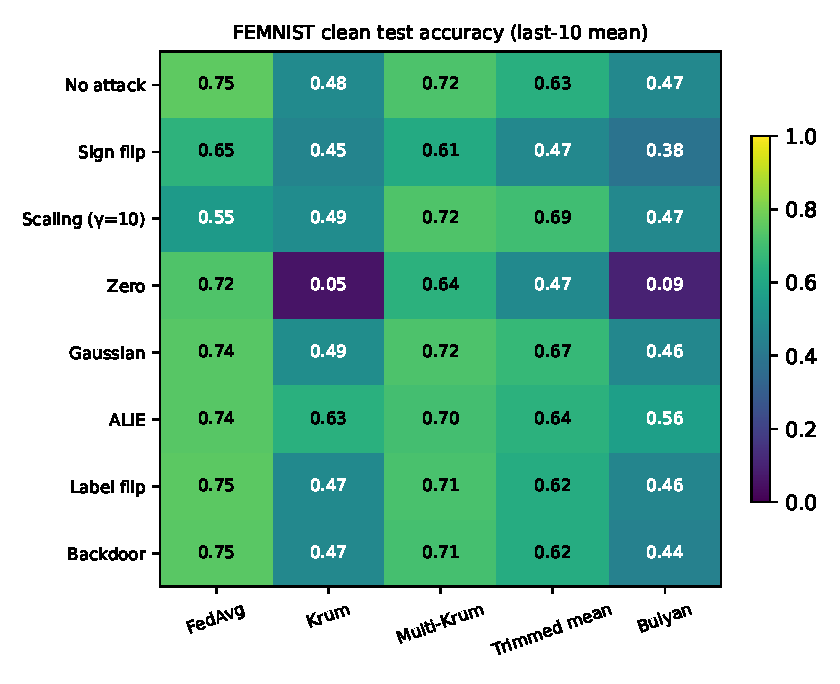
\includegraphics[width=0.8\linewidth]{femnist_heatmap}
\caption{FEMNIST clean test accuracy by attack and defense.}
\label{fig:femnist-heatmap}
\end{figure}

\paragraph{Robustness has a price without an attack.}
With no attack, every robust rule lost accuracy against FedAvg's 0.752. Multi-Krum lost least, at 0.032 (95\% CI 0.007 to 0.058), followed by trimmed mean at 0.123, Krum at 0.274 and Bulyan at 0.284. Krum keeps one client per round and Bulyan rejects about 40\% of honest participants, so a likely reason for their loss is that they discard much of each round's information from non-IID writers. We did not test this explanation.

\paragraph{Which attack matters depends on the rule.}
Scaling with $\gamma=10$ harmed FedAvg badly while leaving a robust rule almost unaffected. FedAvg fell to 0.546, and Multi-Krum held 0.724, a paired gain of 0.178 (95\% CI 0.093 to 0.262). Trimmed mean gained 0.146 (95\% CI 0.039 to 0.253). Sign flip reduced FedAvg to 0.647, yet no robust rule beat it there. Multi-Krum came closest at 0.610, and trimmed mean and Bulyan were hit harder than FedAvg (0.467 and 0.380).

\paragraph{The zero attack stopped Krum.}
Zero was the most damaging attack in the grid, and it did almost nothing to FedAvg, which held 0.723. Krum fell to 0.054 and Bulyan to 0.094. Krum selected a zero update nearly every round: its aggregate was exactly zero in 98 to 99 of 100 rounds on every seed, and it rejected all honest clients over the last 10 rounds (FPR 1.000). The global model barely trained. A likely reason is that the identical zero updates sit near each other and may lie nearer to honest updates than honest updates lie to one another, but we did not measure these distances. Multi-Krum kept every zero update and lost less (0.643), and trimmed mean reached 0.473.

\paragraph{Gaussian replacement was absorbed.}
Multi-Krum rejected every Gaussian update at an FPR of 0.000 and scored 0.722, its honest level. Trimmed mean scored 0.668, above its honest 0.630. FedAvg still led at 0.738, so no robust rule gained accuracy here either. Scaling was the only attack on FEMNIST where any robust rule beat FedAvg.

\paragraph{ALIE and label flipping did not reduce FedAvg's accuracy here.}
FedAvg reached 0.742 under ALIE and 0.750 under label flipping, close to its 0.752 without attack. The label flip rate stayed near zero for every rule (Table~\ref{tab:femnist-flip}). Under these settings, all robust rules scored below FedAvg on both attacks, so for these attacks they cost accuracy and bought none.

\begin{table}[H]
\centering
\caption{Paired difference from FedAvg under the same attack, with a two-sided 95\% $t$ interval on 2 degrees of freedom.}
\label{tab:femnist-paired}
\begin{tabular}{llccc}
\toprule
Attack & Defense & $\Delta$ accuracy vs.\ FedAvg & 95\% CI & Seeds \\
\midrule
No attack & Krum & -0.274 & [-0.325, -0.223] & 3 \\
No attack & Multi-Krum & -0.032 & [-0.058, -0.007] & 3 \\
No attack & Trimmed mean & -0.123 & [-0.161, -0.084] & 3 \\
No attack & Bulyan & -0.284 & [-0.330, -0.238] & 3 \\
Sign flip & Krum & -0.195 & [-0.294, -0.096] & 3 \\
Sign flip & Multi-Krum & -0.036 & [-0.053, -0.020] & 3 \\
Sign flip & Trimmed mean & -0.180 & [-0.278, -0.082] & 3 \\
Sign flip & Bulyan & -0.267 & [-0.458, -0.076] & 3 \\
Scaling ($\gamma=10$) & Krum & -0.059 & [-0.074, -0.044] & 3 \\
Scaling ($\gamma=10$) & Multi-Krum & +0.178 & [+0.093, +0.262] & 3 \\
Scaling ($\gamma=10$) & Trimmed mean & +0.146 & [+0.039, +0.253] & 3 \\
Scaling ($\gamma=10$) & Bulyan & -0.078 & [-0.249, +0.093] & 3 \\
Zero & Krum & -0.669 & [-0.682, -0.657] & 3 \\
Zero & Multi-Krum & -0.080 & [-0.125, -0.036] & 3 \\
Zero & Trimmed mean & -0.250 & [-0.336, -0.164] & 3 \\
Zero & Bulyan & -0.629 & [-0.721, -0.537] & 3 \\
Gaussian & Krum & -0.249 & [-0.326, -0.171] & 3 \\
Gaussian & Multi-Krum & -0.016 & [-0.019, -0.014] & 3 \\
Gaussian & Trimmed mean & -0.070 & [-0.090, -0.050] & 3 \\
Gaussian & Bulyan & -0.275 & [-0.339, -0.212] & 3 \\
ALIE & Krum & -0.108 & [-0.121, -0.095] & 3 \\
ALIE & Multi-Krum & -0.040 & [-0.068, -0.012] & 3 \\
ALIE & Trimmed mean & -0.101 & [-0.124, -0.077] & 3 \\
ALIE & Bulyan & -0.178 & [-0.232, -0.124] & 3 \\
Label flip & Krum & -0.275 & [-0.298, -0.252] & 3 \\
Label flip & Multi-Krum & -0.037 & [-0.057, -0.017] & 3 \\
Label flip & Trimmed mean & -0.129 & [-0.156, -0.102] & 3 \\
Label flip & Bulyan & -0.294 & [-0.341, -0.247] & 3 \\
Backdoor & Krum & -0.279 & [-0.343, -0.215] & 3 \\
Backdoor & Multi-Krum & -0.040 & [-0.086, +0.006] & 3 \\
Backdoor & Trimmed mean & -0.128 & [-0.186, -0.071] & 3 \\
Backdoor & Bulyan & -0.308 & [-0.373, -0.242] & 3 \\
\bottomrule
\end{tabular}

\end{table}

\begin{table}[H]
\centering
\caption{FEMNIST filtering: fraction of malicious participants rejected (TPR).}
\label{tab:femnist-tpr}
\resizebox{\linewidth}{!}{\begin{tabular}{lccccc}
\toprule
Attack & FedAvg & Krum & Multi-Krum & Trimmed mean & Bulyan \\
\midrule
Sign flip & 0.000 $\pm$ 0.000 & 0.983 $\pm$ 0.029 & 0.308 $\pm$ 0.029 & 0.000 $\pm$ 0.000 & 0.483 $\pm$ 0.052 \\
Scaling ($\gamma=10$) & 0.000 $\pm$ 0.000 & 1.000 $\pm$ 0.000 & 0.992 $\pm$ 0.014 & 0.000 $\pm$ 0.000 & 1.000 $\pm$ 0.000 \\
Zero & 0.000 $\pm$ 0.000 & 0.750 $\pm$ 0.000 & 0.000 $\pm$ 0.000 & 0.000 $\pm$ 0.000 & 0.000 $\pm$ 0.000 \\
Gaussian & 0.000 $\pm$ 0.000 & 1.000 $\pm$ 0.000 & 1.000 $\pm$ 0.000 & 0.000 $\pm$ 0.000 & 1.000 $\pm$ 0.000 \\
ALIE & 0.000 $\pm$ 0.000 & 0.825 $\pm$ 0.025 & 0.025 $\pm$ 0.043 & 0.000 $\pm$ 0.000 & 0.017 $\pm$ 0.029 \\
Label flip & 0.000 $\pm$ 0.000 & 0.983 $\pm$ 0.029 & 0.267 $\pm$ 0.014 & 0.000 $\pm$ 0.000 & 0.475 $\pm$ 0.000 \\
Backdoor & 0.000 $\pm$ 0.000 & 0.967 $\pm$ 0.058 & 0.100 $\pm$ 0.050 & 0.000 $\pm$ 0.000 & 0.633 $\pm$ 0.014 \\
\bottomrule
\end{tabular}
}
\end{table}

\begin{table}[H]
\centering
\caption{FEMNIST filtering: fraction of honest participants rejected (FPR).}
\label{tab:femnist-fpr}
\resizebox{\linewidth}{!}{\begin{tabular}{lccccc}
\toprule
Attack & FedAvg & Krum & Multi-Krum & Trimmed mean & Bulyan \\
\midrule
No attack & 0.000 $\pm$ 0.000 & 0.950 $\pm$ 0.000 & 0.200 $\pm$ 0.000 & 0.000 $\pm$ 0.000 & 0.400 $\pm$ 0.000 \\
Sign flip & 0.000 $\pm$ 0.000 & 0.942 $\pm$ 0.007 & 0.173 $\pm$ 0.007 & 0.000 $\pm$ 0.000 & 0.379 $\pm$ 0.013 \\
Scaling ($\gamma=10$) & 0.000 $\pm$ 0.000 & 0.938 $\pm$ 0.000 & 0.002 $\pm$ 0.004 & 0.000 $\pm$ 0.000 & 0.250 $\pm$ 0.000 \\
Zero & 0.000 $\pm$ 0.000 & 1.000 $\pm$ 0.000 & 0.250 $\pm$ 0.000 & 0.000 $\pm$ 0.000 & 0.500 $\pm$ 0.000 \\
Gaussian & 0.000 $\pm$ 0.000 & 0.938 $\pm$ 0.000 & 0.000 $\pm$ 0.000 & 0.000 $\pm$ 0.000 & 0.250 $\pm$ 0.000 \\
ALIE & 0.000 $\pm$ 0.000 & 0.981 $\pm$ 0.006 & 0.244 $\pm$ 0.011 & 0.000 $\pm$ 0.000 & 0.496 $\pm$ 0.007 \\
Label flip & 0.000 $\pm$ 0.000 & 0.942 $\pm$ 0.007 & 0.183 $\pm$ 0.004 & 0.000 $\pm$ 0.000 & 0.381 $\pm$ 0.000 \\
Backdoor & 0.000 $\pm$ 0.000 & 0.946 $\pm$ 0.014 & 0.225 $\pm$ 0.012 & 0.000 $\pm$ 0.000 & 0.342 $\pm$ 0.004 \\
\bottomrule
\end{tabular}
}
\end{table}

\paragraph{Filtering rarely separates clients cleanly.}
Tables~\ref{tab:femnist-tpr} and~\ref{tab:femnist-fpr} show that only scaling and Gaussian replacement are filtered cleanly: Multi-Krum's TPR is 0.992 and 1.000 at FPRs of 0.002 and 0.000. Elsewhere rejection is close to indiscriminate or inverted. Under ALIE, Multi-Krum rejected malicious clients at 0.025 and honest clients at 0.244, and under the zero attack at 0.000 and 0.250, so a malicious client was less likely to be rejected than an honest one. Krum's high TPR reflects that it keeps one client per round, rejecting honest clients at 0.938 or above. Its TPR should not be read as detection. Trimmed mean and FedAvg show zero rejection by construction, so the table says nothing about their robustness.

\begin{table}[H]
\centering
\caption{FEMNIST backdoor attack success rate, last-10-round mean. Krum's seeds were 0.043, 0.060 and 0.977.}
\label{tab:femnist-asr}
\resizebox{\linewidth}{!}{\begin{tabular}{lccccc}
\toprule
Attack & FedAvg & Krum & Multi-Krum & Trimmed mean & Bulyan \\
\midrule
Backdoor & 1.000 $\pm$ 0.000 & 0.360 $\pm$ 0.535 & 1.000 $\pm$ 0.000 & 0.427 $\pm$ 0.186 & 0.130 $\pm$ 0.036 \\
\bottomrule
\end{tabular}
}
\end{table}

\begin{table}[H]
\centering
\caption{FEMNIST label flip rate (source class 1 to target class 7).}
\label{tab:femnist-flip}
\resizebox{\linewidth}{!}{\begin{tabular}{lccccc}
\toprule
Attack & FedAvg & Krum & Multi-Krum & Trimmed mean & Bulyan \\
\midrule
Label flip & 0.005 $\pm$ 0.003 & 0.059 $\pm$ 0.089 & 0.010 $\pm$ 0.003 & 0.012 $\pm$ 0.006 & 0.013 $\pm$ 0.009 \\
\bottomrule
\end{tabular}
}
\end{table}

\begin{figure}[H]
\centering
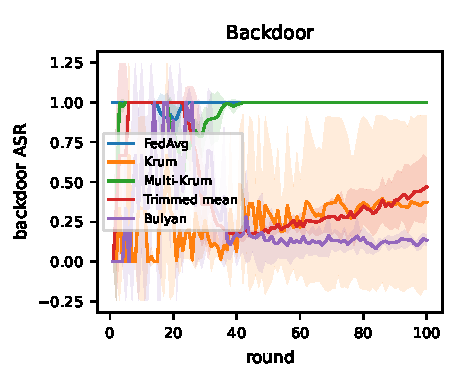
\includegraphics[width=0.6\linewidth]{femnist_asr}
\caption{FEMNIST backdoor attack success rate over rounds; the band is one sample standard deviation.}
\label{fig:femnist-asr}
\end{figure}

\paragraph{Backdoor.}
The backdoor reached an ASR of 1.000 on all three seeds under both FedAvg and Multi-Krum (Table~\ref{tab:femnist-asr}), so Multi-Krum, the best-performing rule on clean accuracy, gave no protection. Bulyan was lowest at 0.130, but with clean accuracy of only 0.438. Trimmed mean reached 0.427 with wide variation. Krum's mean of 0.360 hides a split: two seeds stayed near 0.05 and one reached 0.977. This is one rule on three seeds, and we draw no conclusion about Krum's reliability beyond that spread.

\begin{figure}[H]
\centering
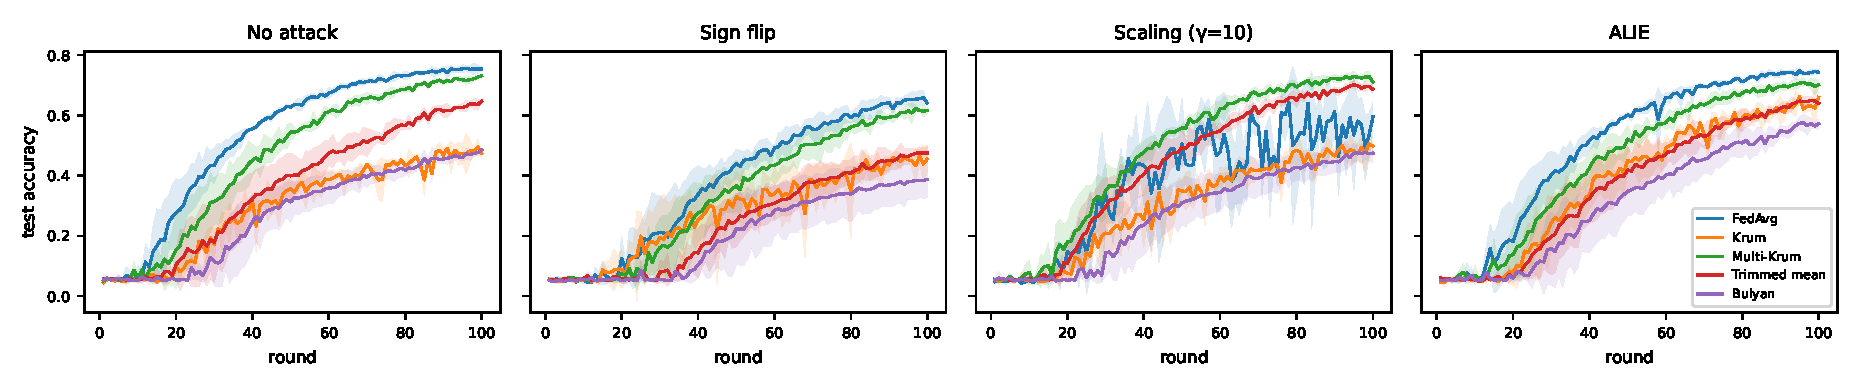
\includegraphics[width=\linewidth]{femnist_curves}
\caption{FEMNIST test accuracy over rounds; the band is one sample standard deviation.}
\label{fig:femnist-curves}
\end{figure}

\subsection{Speech Commands}

Table~\ref{tab:speech-accuracy} gives accuracy on the full test split after 40 rounds, which is not convergence. Only FedAvg, Multi-Krum and trimmed mean ran here, on seeds 0 to 2. Because many cells have diverged seeds, we give no paired intervals.

\begin{table}[H]
\centering
\caption{Speech Commands full-test accuracy after 40 rounds, BC-ResNet-8: mean $\pm$ sample standard deviation over the seeds that finished. ``div.\ round $r$'' gives the round each other seed diverged, and such runs have no accuracy.}
\label{tab:speech-accuracy}
\begin{tabular}{lccc}
\toprule
Attack & FedAvg & Multi-Krum & Trimmed mean \\
\midrule
No attack & 0.497 $\pm$ 0.036 & 0.408 $\pm$ 0.021 & 0.382 $\pm$ 0.027 \\
Sign flip & div.\ round 11, 1, 14 & div.\ round 1, 28, 11 & 0.280 $\pm$ 0.023 \\
Scaling ($\gamma=10$) & div.\ round 1, 1, 1 & 0.325 $\pm$ 0.084; div.\ round 8 & 0.426 $\pm$ 0.051 \\
Backdoor & 0.441 $\pm$ 0.071 & 0.369 $\pm$ 0.040 & 0.349 $\pm$ 0.057 \\
\bottomrule
\end{tabular}

\end{table}

\paragraph{Baseline.}
Without an attack FedAvg scored 0.497, Multi-Krum 0.408 and trimmed mean 0.382. The robust rules cost more here, relative to FedAvg, than Multi-Krum did on FEMNIST, although training was far from converged.

\paragraph{Attacks caused divergence.}
Ten of the 36 runs failed, all with a non-finite evaluation loss. FedAvg diverged in round~1 under scaling on all three seeds, and under sign flip in rounds 11, 1 and 14. Multi-Krum diverged under sign flip in rounds 1, 28 and 11, and under scaling in round~8 of seed~2. No honest run and no trimmed-mean run diverged. We replayed two of these runs, scaling with FedAvg and sign flip with Multi-Krum on seed~0. Both came from a negative BatchNorm running variance in the aggregate, which the simulator refuses to clamp (Section~\ref{sec:limitations}). In the Multi-Krum case a single flipped client passed the filter and left 1 of 128 entries in one layer negative. The other eight were not replayed, so their cause is unverified.

\paragraph{Trimmed mean held on the update attacks.}
Trimmed mean was the only rule to complete all attacks. Under scaling it scored 0.426, above its 0.382 without attack on all three seeds, as it also did on FEMNIST. We did not test why. Sign flip reduced it to 0.280. Multi-Krum finished scaling on two seeds, at 0.266 and 0.385 against 0.408 without attack, though it rejected 0.85 and 1.00 of malicious clients over their last 10 rounds. A scaled update that passes the filter even occasionally may do lasting damage, which could explain the gap, but we did not test this.

\paragraph{Backdoor.}
The feature-space backdoor reached an ASR of at least 0.976 under FedAvg and at least 0.922 under Multi-Krum on every seed (Table~\ref{tab:speech-asr}). Under trimmed mean the seeds disagreed completely, at 0.0004, 0.777 and 0.852, and the seed~0 run had reached 0.831 on the 300-clip in-loop subset before falling to zero. On seed~2 the in-loop value moved between 0.07 and 0.80 in the last six rounds, so a single final score is unstable. Trimmed mean therefore did not reliably stop this backdoor, and its mean of 0.543 describes no seed.

\begin{table}[H]
\centering
\caption{Speech Commands backdoor ASR on the full test split after 40 rounds, over three seeds.}
\label{tab:speech-asr}
\begin{tabular}{lccc}
\toprule
Attack & FedAvg & Multi-Krum & Trimmed mean \\
\midrule
Backdoor & 0.985 $\pm$ 0.008 & 0.959 $\pm$ 0.032 & 0.543 $\pm$ 0.472 \\
\bottomrule
\end{tabular}

\end{table}

